%\chapter{Manhattan: A Case Study in Gentrification}

\section{Manhattan: A Case Study in Gentrification}\label{case_study}

In this section we explore how tracts identified by the Columbia methodology and the tracts identified by our methodology as having been gentrified compare in terms of the change in market value of condominiums along with the effect of the evolving property market, as well as the implications for renters. We consider Manhattan (County of New York), one of the five borough of New York City, as the focus of our study. 

The Department of Finance (DOF) is required by New York state law to value condominiums or cooperatives as though they are residential apartment buildings and these valuations are made public through the DOF Condominium Comparable Rental Income dataset \cite{DOF Condo Valuation dataset} (DOF Condo Valuation). The DOF uses a relative method of valuation combining rental information from similar properties to estimate a market value and more importantly, a market value per square foot which enables comparison between condominiums in different areas regardless of size. The DOF Condo Valuation dataset refers to each property as using a 'Borough, Block, Lot' \cite{BBL info} (BBL) parcel system used in New York City from which we find the GEOID of properties using a tool on the US Census Bureau website \cite{BBL to GEOID conversion}. GEOIDs pertaining to Manhattan are filtered for yielding the dataset used in this case study.

\subsection{Comparing condominium value change in gentrified tracts}
\label{finding excess relative change}

We compare the tracts identified as having undergone gentrification by both the Columbia methodology as well as our own K-means method. The Columbia framework identifies nine tracts as gentrified of which six have sufficient market valuations to proceed. Our framework identifies sixteen gentrified GEOIDs of which two tracts (36061022900, 36061022301) were identified by the Columbia method as well. We compute the mean cumulative percentage change over all GEOIDs for tracts identified by each method in Figure \ref{comparing_cum_perc_change_value}.

However, analysing relative change in property values for gentrified tracts alone doesn't tell us about how prices in these tracts have changed compared to the other, non-gentrified tracts in Manhattan. We calculate the cumulative relative value average for all non-gentrified tracts identified by Columbia and K-means and calculate the excess relative change:

\begin{align}
    R_e = R_g - R_{ng} \\
    R_e,\ \text{Excess relative change} \nonumber \\
    R_g,\ \text{Relative change in gentrified tracts} \nonumber \\
    R_{ng},\ \text{Relative change in non-gentrified tracts} \nonumber
\end{align}

\begin{figure}[h]
    \centering
    \scalebox{0.5}  
    {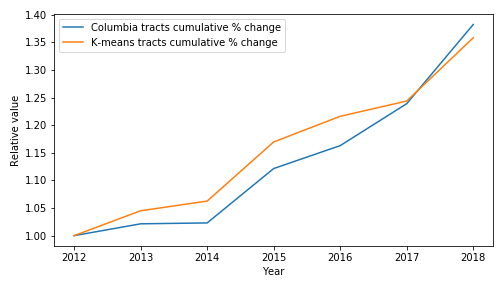
\includegraphics{figs/comparing_rv_in_g_tracts.png}}
    \caption{Comparing cumulative relative change in condominium values}
    \label{comparing_cum_perc_change_value}
\end{figure}

We plot the excess relative change for gentrified tracts identified by each method in Figure \ref{excess_rchange}. We see that the gentrified tracts identified by the Columbia method see very little excess increase over  
non-gentrified tracts up until 2016, after which a sharp increase in excess relative change occurs. The excess change for gentrified tracts identified by K-means, on the other hand, shows a far more gradual but consistent positive excess over non-gentrified tracts. But we are now faced with the question, how does this compare to the state of the general housing market in Manhattan? Specifically, how has the market driven this trend?

\begin{figure}[h]
    \centering
    \scalebox{0.5}  
    {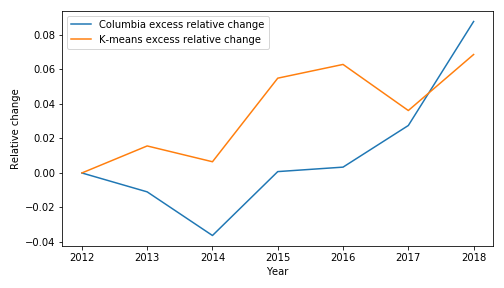
\includegraphics{figs/excess_rchange.png}}
    \caption{Excess relative change in condo prices}
    \label{excess_rchange}
\end{figure}

\subsection{The property market in Manhattan}

We are interested in the broad state of the housing market in New York City and more specifically, Manhattan. The magazine, \textit{New York Curbed}, has performed an analysis of the general property marked in the five boroughs of New York City \cite{Curbed analysis} and openly provides the datasets they used with total property sales per quarter from Q1 2010 to Q3 2019 and mean sale price for Manhattan for the same time frame. Analysing the state of the property market in Manhattan allows us to assess and explain excess relative change observed in the Section \ref{finding excess relative change}. 

Using the aforementioned datasets, we plot the number of sales per quarter for all boroughs in Figure \ref{sales_quarter_borough} where we see Manhattan dominating with most sales in the early half of the 2010's, ceding this title to Queens post approximately 2015. Plotting the relative change in sales for the period we are interested in, 2012-2018, (Figure \ref{manhattan_relative_sales}) we see that sales peak in 2013 and 2014 before generally declining. However, during this period the average sale price of properties in Manhattan has increased monotonically (Figure \ref{manhattan_mean_sale_price}) despite a reduction in overall sales leading to an overall increase in annual market value in Figure \ref{manhattan_market_size}, except for 2018. 

\begin{figure}[H]
    \centering
    \scalebox{0.5}  
    {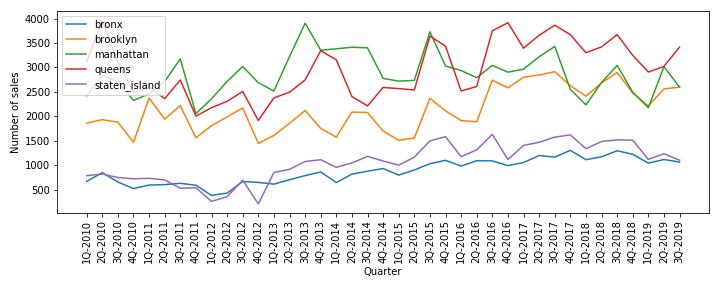
\includegraphics{figs/sales_by_borough_per_quarter.png}}
    \caption{Total sales per quarter}
    \label{sales_quarter_borough}
\end{figure}

\begin{figure}[H]
    \centering
    \scalebox{0.5}  
    {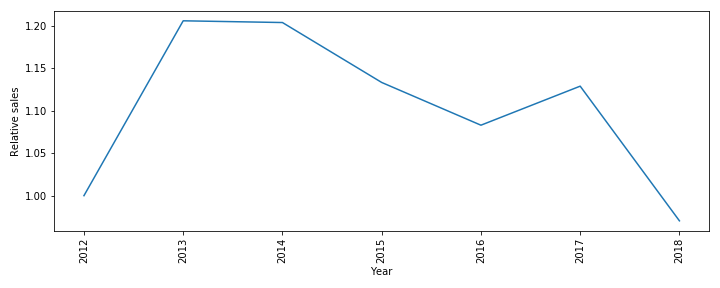
\includegraphics{figs/manhattan_relative_sales.png}}
    \caption{Manhattan relative property sales 2012-2018}
    \label{manhattan_relative_sales}
\end{figure}

\begin{figure}[H]
    \centering
    \scalebox{0.5}  
    {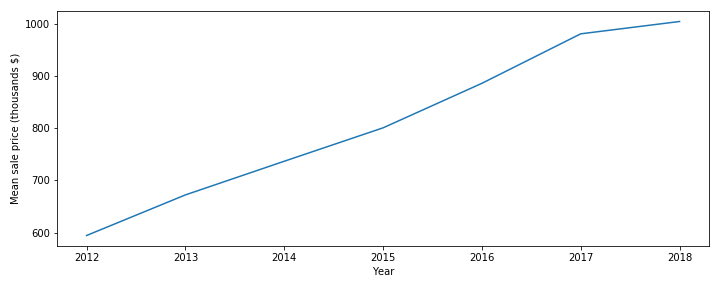
\includegraphics{figs/manhattan_mean_sale_price.png}}
    \caption{Manhattan mean sale price 2012-2018}
    \label{manhattan_mean_sale_price}
\end{figure}

\begin{figure}[H]
    \centering
    \scalebox{0.5}  
    {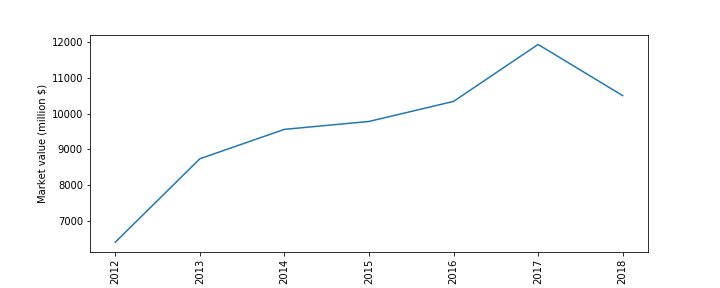
\includegraphics{figs/manhattan_property_market.png}}
    \caption{Manhattan property market value 2012-2018}
    \label{manhattan_market_size}
\end{figure}

2018 saw the worst performing Manhattan real estate market since 2009 as over the past decade \cite{CNBC Manhattan real estate}, lack of available land for new construction led to increasing land values which in turn encouraged any new properties to be built for the luxury market resulting in a lack of more affordable housing. Financial market performance in 2018 saw a souring of interest for Manhattan real estate from foreign investors leading to a declining property market. 

Figure \ref{columbia_summary} shows that condo price growth in areas identified as gentrified according to the Columbia methodology has occurred almost exclusively after 2016, merely two years after the decline in Manhattan's property sales began. This suggests that gentrification in Manhattan is a very recent phenomenon that has occurred in response to dwindling interest in the high value properties. In comparison, condominium prices in areas identified as gentrified by our K-means model (Figure \ref{k_means_summary}) identifies more tracts that have seen excess increase in condo prices far earlier with weak signs of excess increase prior to 2014 and far more significant excess increase after 2014, which corresponds to gentrification as a response to a reduction in property sales. With our K-means method, we are able to identify tracts undergoing gentrification earlier than with the Columbia method, as well as relate gentrification more closely to the state of the property market in the area. 

\begin{figure}[h]
\centering
\begin{subfigure}{.5\textwidth}
  \centering
  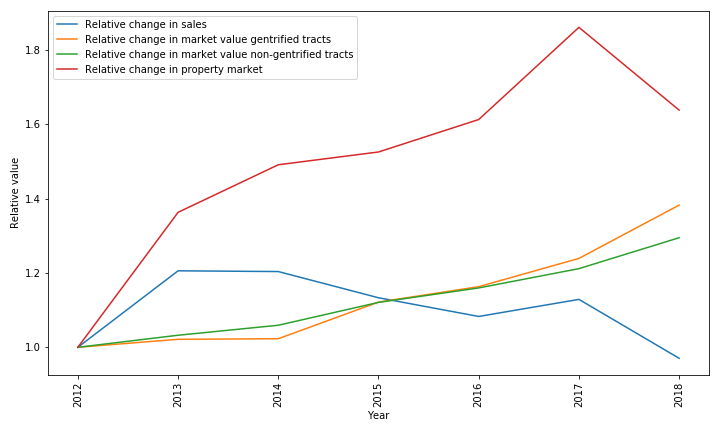
\includegraphics[width=1.0\linewidth]{figs/columbia_summary.png}
  \caption{Columbia method comparative plot}
  \label{columbia_summary}
\end{subfigure}%
\begin{subfigure}{.5\textwidth}
  \centering
  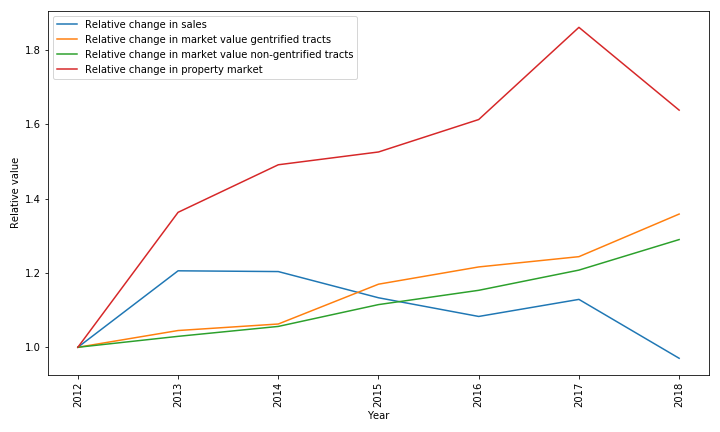
\includegraphics[width=1.0\linewidth]{figs/k_means_summary.png}
  \caption{K-means method comparative plot}
  \label{k_means_summary}
\end{subfigure}
\caption{Comparative plots for Columbia and K-means method results}
\label{methods_summary_plot}
\end{figure}

\subsection{Considering rental properties}

Thus far we have considered only the price of properties -- price is a direct indicator of the desirability and demand for housing in an area -- but we have failed to consider displacement. Renters are another key demographic in an area as they are ones that are likely to be 'priced out' of their homes during the process of gentrification. Yet we disregard this information with good reason; New York only provides data on evictions from the year 2017 \cite{Evictions data}. This limits the extent to which we can use evictions data to identify gentrified tracts, but in this study it provides a crucial way of evaluating the methodologies that find such tracts. 

We consider residential evictions in Manhattan that were completed in 2017 and 2018, although we note that eviction proceedings take on average twelve weeks in New York, in addition to up to six months a judge can award a tenant to stay in a property before eviction.

To enable comparison between evictions in gentrified and non-gentrified areas, we normalise total evictions by the number of GEOID tracts they occurred in thereby obtaining an average evictions per tract metric for 2017 and 2018. 

Figure \ref{columbia_evictions} shows that gentrified tracts identified by the Columbia method show significantly higher eviction rates than non-gentrified tracts with the eviction rate increasing in 2018 for these gentrified tracts. By contrast, in Figure \ref{k_means_evictions}, the K-means method gentrified tracts show a very similar eviction rate with both non-gentrified areas as well as across the two years. This potentially suggests that the Columbia method is more adept at recognising displacement due to gentrification, although more data of evictions throughout the 2012-2018 period would confirm this. 

\begin{figure}[h]
\centering
\begin{subfigure}{.5\textwidth}
  \centering
  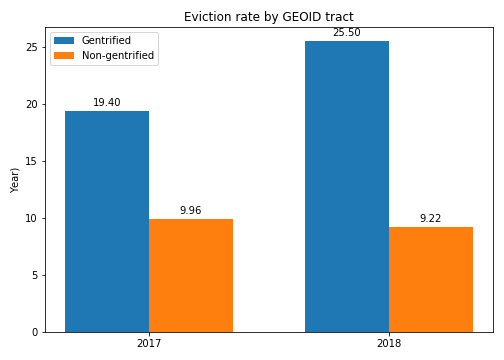
\includegraphics[width=1.0\linewidth]{figs/columbia_evictions.png}
  \caption{Columbia method}
  \label{columbia_evictions}
\end{subfigure}%
\begin{subfigure}{.5\textwidth}
  \centering
  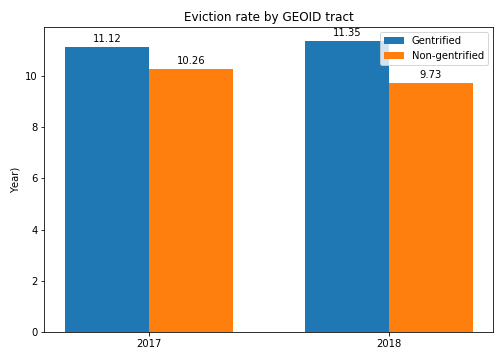
\includegraphics[width=1.0\linewidth]{figs/k_means_evictions.png}
  \caption{Our K-means method}
  \label{k_means_evictions}
\end{subfigure}
\caption{Evictions per tract for gentrified and non-gentrified tracts identified by Columbia and K-means methods}
\label{evictions}
\end{figure}

